\documentclass[11pt]{article}
\usepackage[T1]{fontenc}
\usepackage{lmodern}
\usepackage[a4paper,left=25mm,right=30mm,top=22mm,bottom=24mm,marginparwidth=18mm]{geometry}
\usepackage{amsmath,amssymb,mathtools,stmaryrd}
\usepackage{tikz}
\usetikzlibrary{arrows.meta,calc,positioning}
\usepackage{caption}
\usepackage{xcolor}
\usepackage{marginnote}
\usepackage{microtype}
\usepackage[hidelinks]{hyperref}
\definecolor{LeanTeal}{HTML}{087F72}
\definecolor{SourceGray}{HTML}{66736F}
\setlength{\parindent}{0pt}
\setlength{\parskip}{0.55em}
\setlength{\emergencystretch}{2em}
\newcommand{\leanmarker}[2]{%
  \marginnote{\hyperlink{#1}{\color{LeanTeal}\fbox{\scriptsize Lean}}}%
  \hypertarget{#1}{\textbf{#2.}}%
}
\newcommand{\sourcepage}[1]{\par\medskip\noindent\textcolor{SourceGray}{\scriptsize Source PDF page #1}\par\smallskip}
\pagestyle{plain}
\begin{document}
\begin{center}\LARGE\bfseries Domains individually\par\medskip
\large Lean 4 Formalization Companion -- Chapter 2\end{center}
\medskip
\noindent\textit{This project-generated reading copy contains reviewed mathematical items, short source locators, and redrawn diagrams. It does not reproduce the original PDF or automatic OCR prose. Click a Lean tag in the web reader to open the mapped Lean declaration.}
\bigskip\hrule\bigskip
\section*{Section 2.1}
\sourcepage{10}
\leanmarker{def-2-1-1}{Definition 2.1.1} A set $P$ with a binary relation $\sqsubseteq$ is called a partially ordered set or poset if the following holds for all $x,y,z\in P$:
\begin{enumerate}
\item $x\sqsubseteq x$ (Reflexivity)
\item $x\sqsubseteq y \wedge y\sqsubseteq z \Rightarrow x\sqsubseteq z$ (Transitivity)
\item $x\sqsubseteq y \wedge y\sqsubseteq x \Rightarrow x=y$ (Antisymmetry)
\end{enumerate}
If antisymmetry is omitted, the structure is a preorder. The induced equivalence relation is $\sqsubseteq\cap\sqsupseteq$, and passing to equivalence classes gives a canonical poset. A common way to extract order-theoretic content from a relation $R$ is its transitive closure $\bigcup_{n\in\mathbb{N}\setminus\{0\}} R^n$.

\leanmarker{prop-2-1-2}{Proposition 2.1.2} If $\langle P,\sqsubseteq\rangle$ is an ordered set, then so is $P^{op}=\langle P,\sqsupseteq\rangle$.

\begin{figure}[ht]
\centering
\setlength{\tabcolsep}{1.8em}
\begin{tabular}{ccc}
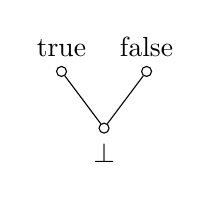
\begin{tikzpicture}[scale=0.72,baseline=(current bounding box.center)]
  \tikzset{dot/.style={circle,draw,fill=white,inner sep=0pt,minimum size=3.6pt}}
  \node[dot,label=above:{true}] (t) at (-0.75,1.0) {};
  \node[dot,label=above:{false}] (f) at (0.75,1.0) {};
  \node[dot,label=below:{$\bot$}] (b) at (0,0) {};
  \draw (b)--(t) (b)--(f);
\end{tikzpicture}
&
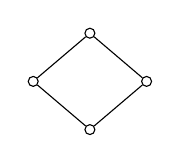
\begin{tikzpicture}[scale=0.72,baseline=(current bounding box.center)]
  \tikzset{dot/.style={circle,draw,fill=white,inner sep=0pt,minimum size=3.6pt}}
  \node[dot] (top) at (0,1.7) {};
  \node[dot] (l) at (-1.0,0.85) {};
  \node[dot] (r) at (1.0,0.85) {};
  \node[dot] (bot) at (0,0) {};
  \draw (bot)--(l)--(top)--(r)--(bot);
\end{tikzpicture}
&
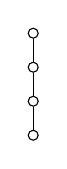
\begin{tikzpicture}[scale=0.72,baseline=(current bounding box.center)]
  \tikzset{dot/.style={circle,draw,fill=white,inner sep=0pt,minimum size=3.6pt}}
  \node[dot] (a) at (0,0) {};
  \node[dot] (b) at (0,0.6) {};
  \node[dot] (c) at (0,1.2) {};
  \node[dot] (d) at (0,1.8) {};
  \draw (a)--(b)--(c)--(d);
\end{tikzpicture}
\\[-0.1em]
The flat booleans & The four-element lattice & The four-element chain
\end{tabular}
\caption*{Figure 1: A few posets drawn as line diagrams.}
\end{figure}

\begin{figure}[ht]
\centering
\setlength{\tabcolsep}{2.1em}
\begin{tabular}{ccc}
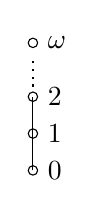
\begin{tikzpicture}[scale=0.72,baseline=(current bounding box.center)]
  \tikzset{dot/.style={circle,draw,fill=white,inner sep=0pt,minimum size=3.4pt}}
  \foreach \y/\lab in {0/0,0.65/1,1.3/2} {\node[dot,label=right:{$\lab$}] at (0,\y) {};}
  \draw (0,0)--(0,1.3);
  \draw[dotted,line width=0.8pt] (0,1.48)--(0,2.02);
  \node[dot,label=right:{$\omega$}] at (0,2.25) {};
\end{tikzpicture}
&
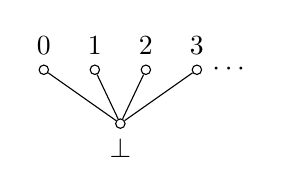
\begin{tikzpicture}[scale=0.72,baseline=(current bounding box.center)]
  \tikzset{dot/.style={circle,draw,fill=white,inner sep=0pt,minimum size=3.4pt}}
  \node[dot,label=below:{$\bot$}] (bot) at (0,0) {};
  \foreach \x/\lab in {-1.35/0,-0.45/1,0.45/2,1.35/3} {
    \node[dot,label=above:{$\lab$}] (p\lab) at (\x,0.95) {};
    \draw (bot)--(p\lab);
  }
  \node at (1.95,0.95) {$\cdots$};
\end{tikzpicture}
&
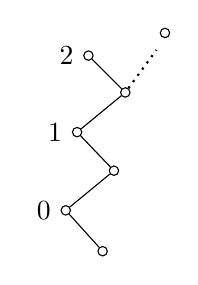
\begin{tikzpicture}[scale=0.72,baseline=(current bounding box.center)]
  \tikzset{dot/.style={circle,draw,fill=white,inner sep=0pt,minimum size=3.4pt}}
  \node[dot] (b0) at (0,0) {};
  \node[dot,label=left:{$0$}] (z) at (-0.65,0.72) {};
  \node[dot] (b1) at (0.2,1.42) {};
  \node[dot,label=left:{$1$}] (o) at (-0.45,2.1) {};
  \node[dot] (b2) at (0.4,2.8) {};
  \node[dot,label=left:{$2$}] (t) at (-0.25,3.45) {};
  \draw (b0)--(z)--(b1)--(o)--(b2)--(t);
  \draw[dotted,line width=0.8pt] (b2)--(0.95,3.55);
  \node[dot] at (1.1,3.85) {};
\end{tikzpicture}
\\[-0.1em]
ordinal & flat & lazy
\end{tabular}
\caption*{Figure 2: Three versions of the natural numbers.}
\end{figure}

\begin{figure}[ht]
\centering
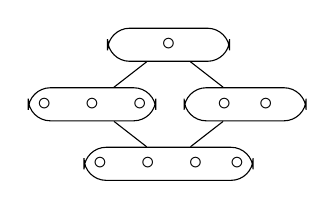
\begin{tikzpicture}[scale=0.72]
  \tikzset{class/.style={draw,rounded corners=8pt,minimum width=1.55cm,minimum height=0.42cm}, dot/.style={circle,draw,fill=white,inner sep=0pt,minimum size=3.0pt}}
  \node[class] (top) at (0,2.1) {$\circ$};
  \node[class] (left) at (-1.35,1.05) {$\circ\quad\circ\quad\circ$};
  \node[class] (right) at (1.35,1.05) {$\circ\quad\circ$};
  \node[class] (bot) at (0,0) {$\circ\quad\circ\quad\circ\quad\circ$};
  \draw (bot)--(left)--(top)--(right)--(bot);
\end{tikzpicture}
\caption*{Figure 3: A preorder whose canonical quotient is the four-element lattice.}
\end{figure}

\sourcepage{11}
\leanmarker{def-2-1-3}{Definition 2.1.3} Let $(P,\sqsubseteq)$ be an ordered set.
\begin{enumerate}
\item A subset $A$ of $P$ is an upper set if $x\in A$ and $y\sqsupseteq x$ imply $y\in A$. We write $\uparrow A$ for the set of elements above some element of $A$, and abbreviate $\uparrow\{x\}$ as $\uparrow x$. The dual notions are lower set and $\downarrow A$.
\item An element $x\in P$ is an upper bound for $A\subseteq P$ if every element of $A$ is below $x$; we write $A\sqsubseteq x$. The sets of upper and lower bounds are denoted $\operatorname{ub}(A)$ and $\operatorname{lb}(A)$.
\item An element $x\in P$ is maximal if $\uparrow x\cap P=\{x\}$. Minimal elements are defined dually. Minimal upper bounds of $A$ are collected in $\operatorname{mub}(A)$.
\item If all elements of $P$ are below a single element $x\in P$, then $x$ is the largest element. The dually defined least element is also called bottom and is denoted $\bot$.
\item If $A\subseteq P$ has a least upper bound $x$, then $x$ is the supremum or join of $A$, written $x=\bigvee A$. Dually, an infimum or meet is written $x=\bigwedge A$.
\item A poset is a $\sqcup$-semilattice, respectively $\sqcap$-semilattice, if each pair has a supremum, respectively infimum. It is a lattice if both operations exist, and complete if suprema and infima exist for all subsets.
\end{enumerate}

\sourcepage{12}
\leanmarker{prop-2-1-4}{Proposition 2.1.4} Let $P$ be a poset such that the suprema and infima occurring below exist. Let $A,B$ and all $A_i$ be subsets of $P$.
\begin{enumerate}
\item If $A\subseteq B$, then $\bigvee A\sqsubseteq \bigvee B$ and $\bigwedge A\sqsupseteq \bigwedge B$.
\item $\bigvee A=\bigvee(\downarrow A)$ and $\bigwedge A=\bigwedge(\uparrow A)$.
\item If $A=\bigcup_{i\in I} A_i$, then
\[
  \bigvee A = \bigvee_{i\in I}\bigl(\bigvee A_i\bigr),
\]
and similarly for the infimum.
\end{enumerate}
\emph{Proof.} For (3), $\bigvee A$ is above every $A_i$, hence above each $\bigvee A_i$. Conversely, each $a\in A$ belongs to some $A_i$, so it is below $\bigvee A_i$ and therefore below $\bigvee_i(\bigvee A_i)$. This proves the displayed equality; the infimum statement is dual.

\leanmarker{prop-2-1-5}{Proposition 2.1.5} Every closure system is a complete lattice with respect to inclusion. Infima are given by intersections; the supremum of a family is the closure of its union.

\sourcepage{13}
\leanmarker{def-2-1-6}{Definition 2.1.6} Let $P$ and $Q$ be partially ordered sets. A function $f:P\to Q$ is called monotone if, for all $x,y\in P$,
\[
  x\sqsubseteq y \quad\Rightarrow\quad f(x)\sqsubseteq f(y).
\]
The set $[P\xrightarrow{m}Q]$ of monotone functions is ordered pointwise: $f\sqsubseteq g$ iff $f(x)\sqsubseteq g(x)$ for all $x\in P$.

\leanmarker{prop-2-1-7}{Proposition 2.1.7} If $L$ is a complete lattice, then every monotone map $f:L\to L$ has a fixed point. The least fixed point is
\[
  \bigwedge\{x\in L \mid f(x)\sqsubseteq x\},
\]
and the greatest fixed point is
\[
  \bigvee\{x\in L \mid x\sqsubseteq f(x)\}.
\]
\emph{Proof.} Let
\[
  A=\{x\in L\mid f(x)\sqsubseteq x\},\qquad a=\bigwedge A.
\]
For every $x\in A$ we have $a\sqsubseteq x$, hence $f(a)\sqsubseteq f(x)\sqsubseteq x$. Taking the infimum over $A$ gives $f(a)\sqsubseteq a$, so $a\in A$. Monotonicity then gives $f(a)\in A$, and therefore $a\sqsubseteq f(a)$. Thus $f(a)=a$, and $a$ is the least fixed point. The greatest fixed point is obtained dually from $\bigvee\{x\in L\mid x\sqsubseteq f(x)\}$.

For lattices, the converse is also true: the existence of fixed points for monotone maps implies completeness. The proof is harder and relies on the Axiom of Choice; see Markowsky.

\leanmarker{def-2-1-8}{Definition 2.1.8} Let $P$ be a poset. A subset $A$ of $P$ is directed if it is nonempty and each pair of elements of $A$ has an upper bound in $A$. If a directed set $A$ has a supremum, it is denoted by $\bigvee^{\uparrow}A$. Directed lower sets are called ideals; ideals of the form $\downarrow x$ are principal. Dually one obtains filtered sets and filters. Chains are nonempty totally ordered subsets, and subsets isomorphic to the natural numbers are called $\omega$-chains.

\leanmarker{prop-2-1-9}{Proposition 2.1.9} Let $A$ be a nonempty subset of a $\sqcup$-semilattice for which $\bigvee A$ exists. Then the join of $A$ can also be written as the directed join
\[
  \bigvee A
  = \bigvee
    \left\{\bigvee M \;\middle|\; M\subseteq A,\ M\text{ finite and nonempty}\right\}.
\]

\sourcepage{14}
\leanmarker{def-2-1-10}{Definition 2.1.10} A monotone net in a poset $P$ is a monotone function $\alpha:I\to P$ from a directed set $I$ into $P$; $I$ is called the index set. If $\alpha:I\to P$ is a monotone net and $\beta:J\to I$ is monotone, with $J$ directed and cofinal in the sense that for every $i\in I$ there is $j\in J$ with $\beta(j)\ge i$, then $\alpha\circ\beta:J\to P$ is called a subnet of $\alpha$. A monotone net has a supremum in $P$ when the set $\{\alpha(i)\mid i\in I\}$ has a supremum in $P$.

\leanmarker{lemma-2-1-11}{Lemma 2.1.11} Let $P$ be a poset and let $\alpha:I\to P$ be a monotone net. Then $\alpha$ has a subnet $\alpha\circ\beta:J\to P$ whose index set $J$ is a lattice and in which every principal ideal is finite.

For the construction, take $J$ to be the set of finite subsets of $I$. Define $\beta:J\to I$ by induction on cardinality:
\[
\beta(\emptyset)=\text{any element of }I,
\]
and, for $A\ne\emptyset$,
\[
\beta(A)=\text{any upper bound of }A\cup\{\beta(B)\mid B\subset A\}.
\]
Then $\beta$ is monotone and cofinal, hence defines the required subnet.

\leanmarker{prop-2-1-12}{Proposition 2.1.12} Let $I$ be directed and let $\alpha:I\times I\to P$ be a monotone net. Assuming the indicated directed suprema exist, the iterated suprema and the diagonal supremum agree:
\[
\bigvee
  \{\alpha(i,j)\mid i,j\in I\}
=\bigvee_{i\in I}^{\uparrow}\left(\bigvee_{j\in I}^{\uparrow}\alpha(i,j)\right)
=\bigvee_{j\in I}^{\uparrow}\left(\bigvee_{i\in I}^{\uparrow}\alpha(i,j)\right)
=\bigvee_{i\in I}^{\uparrow}\alpha(i,i).
\]

\sourcepage{15}
\leanmarker{def-2-1-13}{Definition 2.1.13} A poset $D$ is called a directed-complete partial order, or dcpo, if every directed subset of $D$ has a supremum.

\textbf{Examples 2.1.14.} Every complete lattice is a dcpo; every finite poset is a dcpo; the natural numbers with the usual order are not a dcpo unless a top element is added. Further examples include point sets of locales ordered by specialization.

\leanmarker{prop-2-1-15}{Proposition 2.1.15} A partially ordered set $D$ is a dcpo if and only if each chain in $D$ has a supremum.

The proof uses the Axiom of Choice and goes back to a lemma of Iwamura; the cited reference is Markowsky.

\leanmarker{prop-2-1-16}{Proposition 2.1.16} A pointed poset $P$ is a dcpo if and only if every monotone map $P\to P$ has a least fixed point.

\leanmarker{def-2-1-17}{Definition 2.1.17} Let $D$ and $E$ be dcpos. A function $f:D\to E$ is \emph{Scott-continuous} if it is monotone and preserves directed suprema: for every directed subset $A\subseteq D$,
\[
  f\left(\bigvee^{\uparrow} A\right)=\bigvee^{\uparrow} f(A).
\]
The continuous functions from $D$ to $E$, ordered pointwise, are denoted $[D\to E]$. A function between pointed dcpos is \emph{strict} if it preserves bottom; continuous strict functions are denoted $[D\xrightarrow{\bot!}E]$. The identity on $A$ is written $\operatorname{id}_A$, and the constant function with value $x$ is written $c_x$.

\sourcepage{16}
\leanmarker{prop-2-1-18}{Proposition 2.1.18} Let $D$ and $E$ be dcpos. Then $[D\to E]$ is again a dcpo. Directed suprema in $[D\to E]$ are calculated pointwise.

\emph{Proof.} Let $F$ be a directed collection of continuous functions from $D$ to $E$. Define
\[
  g(x)=\bigvee_{f\in F}^{\uparrow} f(x).
\]
For a directed set $A\subseteq D$ one computes
\[
\begin{aligned}
  g\left(\bigvee^{\uparrow}A\right)
  &= \bigvee_{f\in F}^{\uparrow} f\left(\bigvee^{\uparrow}A\right) \\
  &= \bigvee_{f\in F}^{\uparrow}\bigvee_{a\in A}^{\uparrow} f(a) && \text{(continuity of $f$)} \\
  &= \bigvee_{a\in A}^{\uparrow}\bigvee_{f\in F}^{\uparrow} f(a) && \text{(Proposition 2.1.12)} \\
  &= \bigvee_{a\in A}^{\uparrow} g(a).
\end{aligned}
\]
Thus $g$ is continuous.

\leanmarker{thm-2-1-19}{Theorem 2.1.19} Let $D$ be a pointed dcpo.
\begin{enumerate}
\item Every continuous function $f:D\to D$ has a least fixed point, namely
\[
  \operatorname{fix}(f)=\bigvee_{n\in\mathbb{N}}^{\uparrow} f^n(\bot).
\]
\item The assignment
\[
  \operatorname{fix}:[D\to D]\to D,
  \qquad f\mapsto \bigvee_{n\in\mathbb{N}}^{\uparrow} f^n(\bot),
\]
is continuous.
\end{enumerate}
The first part is the Kleene fixed point theorem: the iterates form an increasing chain, continuity makes the supremum a fixed point, and induction shows it is below every other fixed point. The second part follows because the iteration operators $\operatorname{it}_n(f)=f^n(\bot)$ are continuous and $\operatorname{fix}$ is their pointwise supremum.

\sourcepage{17}
\leanmarker{lemma-2-1-20}{Lemma 2.1.20} Let $D$ be a dcpo, let $P\subseteq D$ be an admissible predicate, and let $f:D\to D$ be Scott-continuous. If $f(x)$ satisfies $P$ whenever $x$ satisfies $P$, then $\operatorname{fix}(f)$ satisfies $P$.

\leanmarker{lemma-2-1-21}{Lemma 2.1.21} Let $D$ and $E$ be pointed dcpos, let $f:D\to D$ and $g:E\to E$ be continuous, and let $h:D\to E$ be strict and continuous. If the square commutes, $h\circ f=g\circ h$, then
\[
  \operatorname{fix}(g)=h(\operatorname{fix}(f)).
\]
Indeed,
\[
\begin{aligned}
  h(\operatorname{fix}(f))
  &= h\left(\bigvee_{n\in\mathbb{N}}^{\uparrow} f^n(\bot)\right) \\
  &= \bigvee_{n\in\mathbb{N}}^{\uparrow} h(f^n(\bot)) \\
  &= \bigvee_{n\in\mathbb{N}}^{\uparrow} g^n(h(\bot)) \\
  &= \operatorname{fix}(g),
\end{aligned}
\]
using continuity of $h$, commutativity, and strictness of $h$.

\clearpage
\section*{Section 2.2}
\sourcepage{18}
\leanmarker{def-2-2-1}{Definition 2.2.1} Let $x$ and $y$ be elements of a dcpo $D$. We say that $x$ \emph{approximates} $y$, written $x\ll y$, if for every directed subset $A\subseteq D$,
\[
  y\sqsubseteq \bigvee^{\uparrow} A
  \quad\Rightarrow\quad
  \exists a\in A,\ x\sqsubseteq a.
\]
The element $x$ is \emph{compact} if $x\ll x$. For $x,y\in D$ and $A\subseteq D$ the standard notation is
\[
\begin{array}{rcl}
  x\ll y &\Longleftrightarrow& x\text{ approximates }y,\\
  \Downarrow x &=& \{y\in D\mid y\ll x\},\\
  \Uparrow x &=& \{y\in D\mid x\ll y\},\\
  \Uparrow A &=& \displaystyle\bigcup_{a\in A}\Uparrow a,\\
  K(D) &=& \{x\in D\mid x\text{ compact}\}.
\end{array}
\]

\leanmarker{prop-2-2-2}{Proposition 2.2.2} Let $D$ be a dcpo. For all $x,x',y,y'\in D$:
\begin{enumerate}
\item $x\ll y \Rightarrow x\sqsubseteq y$.
\item $x'\sqsubseteq x\ll y\sqsubseteq y' \Rightarrow x'\ll y'$.
\end{enumerate}

\leanmarker{def-2-2-3}{Definition 2.2.3} A subset $B$ of a dcpo $D$ is a \emph{basis} for $D$ if, for every element $x\in D$, the set
\[
  B_x=\Downarrow x\cap B
\]
contains a directed subset with supremum $x$. Elements of $B_x$ are called approximants to $x$ relative to $B$.

\leanmarker{prop-2-2-4}{Proposition 2.2.4} Let $D$ be a dcpo with basis $B$.
\begin{enumerate}
\item For every $x\in D$, the set $B_x$ is directed and
\[
  x=\bigvee^{\uparrow} B_x.
\]
\item $B$ contains $K(D)$.
\item Every superset of $B$ is also a basis for $D$.
\end{enumerate}
\emph{Proof.} For (1), the supremum is clear from the definition; directedness follows by comparing any two approximants with a directed subset of $B_x$ whose supremum is $x$. For (2), if $c\in K(D)$, then from $c=\bigvee^{\uparrow}B_c$ compactness gives some $b\in B_c$ above $c$, while all elements of $B_c$ are below $c$, so $b=c$. Part (3) is immediate from the definition.

\sourcepage{19}
\leanmarker{cor-2-2-5}{Corollary 2.2.5} Let $D$ be a dcpo with basis $B$.
\begin{enumerate}
\item The largest basis for $D$ is $D$ itself.
\item $B$ is the smallest basis for $D$ if and only if $B=K(D)$.
\end{enumerate}
The reverse direction in (2) is not a direct consequence of Proposition 2.2.4; the book leaves it as Exercise 2.3.9(26).

\leanmarker{def-2-2-6}{Definition 2.2.6} A dcpo is \emph{continuous}, or a continuous domain, if it has a basis. It is \emph{algebraic}, or an algebraic domain, if it has a basis of compact elements. It is $\omega$-continuous if it has a countable basis, and $\omega$-algebraic if $K(D)$ is a countable basis.

\leanmarker{prop-2-2-7}{Proposition 2.2.7}
\begin{enumerate}
\item A dcpo $D$ is continuous if and only if, for every $x\in D$,
\[
  x=\bigvee^{\uparrow}\Downarrow x.
\]
\item A dcpo $D$ is algebraic if and only if, for every $x\in D$,
\[
  x=\bigvee^{\uparrow} K(D)_x.
\]
\end{enumerate}

\leanmarker{def-2-2-8}{Definition 2.2.8} A closure system $L$ is called \emph{inductive} if it is closed under directed unions.

\leanmarker{prop-2-2-9}{Proposition 2.2.9} Every inductive closure system $L$ is an algebraic lattice. Its compact elements are precisely the finitely generated hulls.

\emph{Proof.} If $A$ is the hull of a finite set $M$ and $(B_i)_{i\in I}$ is a directed family of hulls with
\[
  \bigvee_{i\in I}^{\uparrow} B_i=\bigcup_{i\in I}B_i\supseteq A,
\]
then $M$ is contained in some $B_i$. Hence finitely generated hulls are compact. Conversely, every closed set is the directed union of finitely generated hulls, so these hulls form a basis; Proposition 2.2.4(2) rules out any other compact elements.

\begin{figure}[ht]
\centering
\setlength{\tabcolsep}{2.6em}
\begin{tabular}{cc}
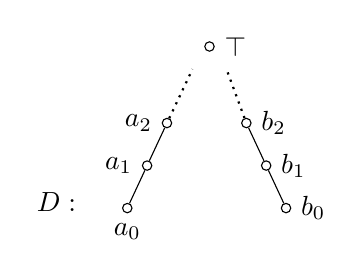
\begin{tikzpicture}[scale=0.72,baseline=(current bounding box.center)]
  \tikzset{dot/.style={circle,draw,fill=white,inner sep=0pt,minimum size=3.4pt}}
  \node at (-2.45,0.1) {$D:$};
  \node[dot,label=below:{$a_0$}] (a0) at (-1.2,0) {};
  \node[dot,label=left:{$a_1$}] (a1) at (-0.85,0.75) {};
  \node[dot,label=left:{$a_2$}] (a2) at (-0.5,1.5) {};
  \draw (a0)--(a1)--(a2);
  \draw[dotted,line width=0.8pt] (a2)--(-0.05,2.45);
  \node[dot,label=right:{$\top$}] (top) at (0.25,2.85) {};
  \node[dot,label=right:{$b_2$}] (b2) at (0.9,1.5) {};
  \node[dot,label=right:{$b_1$}] (b1) at (1.25,0.75) {};
  \node[dot,label=right:{$b_0$}] (b0) at (1.6,0) {};
  \draw (b0)--(b1)--(b2);
  \draw[dotted,line width=0.8pt] (b2)--(0.55,2.45);
\end{tikzpicture}
&
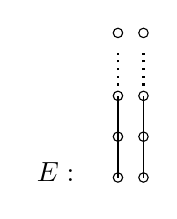
\begin{tikzpicture}[scale=0.72,baseline=(current bounding box.center)]
  \tikzset{dot/.style={circle,draw,fill=white,inner sep=0pt,minimum size=3.4pt}}
  \node at (-1.1,0.1) {$E:$};
  \foreach \x in {0,0.45} {
    \node[dot] at (\x,0) {};
    \node[dot] at (\x,0.72) {};
    \node[dot] at (\x,1.44) {};
    \draw (\x,0)--(\x,1.44);
    \draw[dotted,line width=0.8pt] (\x,1.62)--(\x,2.2);
    \node[dot] at (\x,2.55) {};
  }
\end{tikzpicture}
\end{tabular}
\caption*{Figure 4: A continuous ($E$) and a non-continuous ($D$) dcpo.}
\end{figure}

\begin{figure}[ht]
\centering
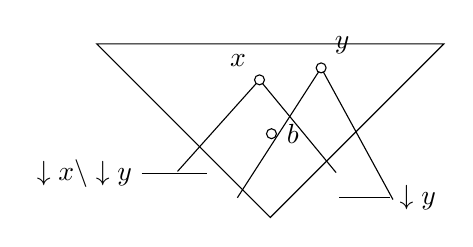
\begin{tikzpicture}[scale=0.76]
  \tikzset{dot/.style={circle,draw,fill=white,inner sep=0pt,minimum size=3.6pt}}
  \draw (-2.9,1.85)--(0,-1.05)--(2.9,1.85)--cycle;
  \draw (-1.55,-0.28)--(-0.18,1.25)--(1.1,-0.3);
  \draw (-0.55,-0.72)--(0.85,1.45)--(2.05,-0.75);
  \node[dot,label=above left:{$x$}] at (-0.18,1.25) {};
  \node[dot,label=above right:{$y$}] at (0.85,1.45) {};
  \node[dot,label=right:{$b$}] at (0.02,0.35) {};
  \draw (-2.15,-0.32)--(-1.05,-0.32);
  \node[left] at (-2.15,-0.32) {$\downarrow x\setminus\downarrow y$};
  \draw (1.15,-0.72)--(2.0,-0.72);
  \node[right] at (2.0,-0.72) {$\downarrow y$};
\end{tikzpicture}
\caption*{Figure 5: Basis element $b$ witnesses that $x$ is not below $y$.}
\end{figure}

\sourcepage{21}
\leanmarker{prop-2-2-10}{Proposition 2.2.10} Let $D$ be a continuous domain with basis $B$, and let $x,y\in D$. The following are equivalent:
\[
  x\sqsubseteq y,
  \qquad B_x\subseteq B_y,
  \qquad B_x\subseteq \downarrow y.
\]
Equivalently, if $x\not\sqsubseteq y$, then there exists $b\in B_x$ with $b\not\sqsubseteq y$. Figure 5 depicts this situation.

In the light of Proposition 2.2.10, the dcpo $D$ in Figure 4 is not continuous because the natural would-be basis consisting of the $a_i$'s and $b_i$'s cannot see that
\[
  \bigvee_{n\in\mathbb{N}}^{\uparrow} a_n
  =\bigvee_{n\in\mathbb{N}}^{\uparrow} b_n
  =\top.
\]
In a continuous domain this information would already be reflected by the basis. This is why the continuous version should look like $E$ in Figure 4, which is indeed algebraic.

Bases also allow us to express continuity of functions in a form reminiscent of the $\epsilon$-$\delta$ definition for real-valued functions.

\sourcepage{22}
\leanmarker{prop-2-2-11}{Proposition 2.2.11} Let $f:D\to E$ be a map between continuous domains with bases $B$ and $C$, respectively. Then $f$ is continuous if and only if, for every $x\in D$ and every $e\in C_{f(x)}$, there exists $d\in B_x$ such that
\[
  f(\uparrow d)\subseteq \uparrow e.
\]
\emph{Proof.} If $f$ is continuous, then
\[
  f(x)=f\left(\bigvee^{\uparrow}B_x\right)
      =\bigvee_{d\in B_x}^{\uparrow} f(d).
\]
Since $e\ll f(x)$, some $d\in B_x$ satisfies $e\sqsubseteq f(d)$; monotonicity gives $f(\uparrow d)\subseteq\uparrow e$.

Conversely, first suppose $x\sqsubseteq y$ but $f(x)\not\sqsubseteq f(y)$. By Proposition 2.2.10 choose $e\in C_{f(x)}\setminus\downarrow f(y)$, and then $d\in B_x$ with $f(\uparrow d)\subseteq\uparrow e$. Since $y\in\uparrow d$, this contradicts $e\not\sqsubseteq f(y)$. Thus $f$ is monotone. Now let $A\subseteq D$ be directed with $x=\bigvee^{\uparrow}A$. Monotonicity gives $\bigvee^{\uparrow}f(A)\sqsubseteq f(x)$. If the reverse inequality failed, Proposition 2.2.10 would give $e\in C_{f(x)}$ with $e\not\sqsubseteq\bigvee^{\uparrow}f(A)$; choose $d\in B_x$ with $f(\uparrow d)\subseteq\uparrow e$. Since $d\ll x$, some $a\in A$ lies above $d$, hence $\bigvee^{\uparrow}f(A)\sqsupseteq f(a)\sqsupseteq f(d)\sqsupseteq e$, a contradiction.

This criterion is followed by a fixed-point result for countable bases: a continuous function need not preserve compactness or the order of approximation, so the naive sequence $\bot,f(\bot),f(f(\bot)),\ldots$ need not consist of basis elements.

\leanmarker{prop-2-2-12}{Proposition 2.2.12} Let $D$ be a pointed $\omega$-continuous domain with basis $B$, and let $f:D\to D$ be continuous. Then there exists an $\omega$-chain
\[
  b_0\sqsubseteq b_1\sqsubseteq b_2\sqsubseteq\cdots
\]
of basis elements satisfying:
\begin{enumerate}
\item $b_0=\bot$;
\item for all $n\in\mathbb{N}$, $b_{n+1}\sqsubseteq f(b_n)$;
\item
\[
  \bigvee_{n\in\mathbb{N}}^{\uparrow} b_n
  =\operatorname{fix}(f)
  =\bigvee_{n\in\mathbb{N}}^{\uparrow} f^n(\bot).
\]
\end{enumerate}
The book cites Abramsky for the proof.

\leanmarker{prop-2-2-13}{Proposition 2.2.13} If a dcpo $D$ has a countable basis, then every directed subset of $D$ contains an $\omega$-chain with the same supremum.

This motivates a parallel $\omega$-chain presentation: an $\omega$-ccpo has suprema of all $\omega$-chains; an $\omega$-continuous map preserves those suprema; and $x$ $\omega$-approximates $y$ if
\[
  y\sqsubseteq\bigvee_{n\in\mathbb{N}}^{\uparrow}a_n
  \quad\Rightarrow\quad
  \exists n\in\mathbb{N},\ x\sqsubseteq a_n.
\]
With a countable basis, this version agrees with the directed-set presentation.

\sourcepage{23}
\leanmarker{prop-2-2-14}{Proposition 2.2.14}
\begin{enumerate}
\item Every continuous $\omega$-ccpo is a continuous dcpo.
\item Every algebraic $\omega$-ccpo is an algebraic dcpo.
\item Every $\omega$-continuous map between continuous $\omega$-ccpos is continuous.
\end{enumerate}
\emph{Proof.} Enumerate a countable basis $B$ as $(b_n)_{n\in\mathbb{N}}$. For a directed subset $A$, construct an $\omega$-chain $(a_n)_{n\in\mathbb{N}}$ in $A$ that successively dominates the relevant basis elements below members of $A$. The resulting chain need not be cofinal in $A$, but it has the same supremum because both dominate the same basis elements. This also identifies $\omega$-approximation with ordinary approximation in a continuous $\omega$-ccpo, yielding (1); part (2) follows from the same argument. For (3), if $f$ is $\omega$-continuous and $A$ is directed, choose such an $\omega$-chain $(a_n)$ in $A$. Then
\[
  f\left(\bigvee^{\uparrow}A\right)
  = f\left(\bigvee_{n\in\mathbb{N}}^{\uparrow}a_n\right)
  = \bigvee_{n\in\mathbb{N}}^{\uparrow}f(a_n)
  \sqsubseteq \bigvee^{\uparrow}f(A),
\]
while the opposite inequality follows from monotonicity.

\sourcepage{24}
\leanmarker{lemma-2-2-15}{Lemma 2.2.15} Let $D$ be a continuous domain and let $M\subseteq D$ be a finite set whose elements all approximate $y$. Then there exists $y'\in D$ such that
\[
  M\ll y'\ll y,
\]
meaning $m\ll y'$ for every $m\in M$ and $y'\ll y$. If $B$ is a basis for $D$, then $y'$ may be chosen from $B$.

\emph{Proof.} Define
\[
  A=\{a\in D\mid \exists a'\in D,\ a\ll a'\ll y\}.
\]
The set $A$ is nonempty and directed. Indeed, from $a\ll a'\ll y$ and $b\ll b'\ll y$, directedness of $\Downarrow y$ gives $c'$ above $a'$ and $b'$ with $c'\ll y$; directedness of $\Downarrow c'$ gives $c$ above $a$ and $b$ with $c\ll c'$. Moreover
\[
  \bigvee^{\uparrow}A=y,
\]
because every $y'\ll y$ satisfies $\Downarrow y'\subseteq A$, while all elements of $A$ are below $y$. For each $m\in M$, choose $a_m\in A$ with $m\sqsubseteq a_m$, and let $a\in A$ be an upper bound of the finite family $(a_m)_{m\in M}$. By definition of $A$, some $a'$ satisfies $a\ll a'\ll y$, and this $a'$ interpolates between $M$ and $y$. The basis-refined version is obtained by allowing only basis elements in $A$.

\sourcepage{25}
\leanmarker{cor-2-2-16}{Corollary 2.2.16} Let $D$ be a continuous domain with basis $B$, and let $A\subseteq D$ be directed. If $c\ll\bigvee^{\uparrow}A$, then $c\ll a$ for some $a\in A$. Equivalently,
\[
  \Downarrow\left(\bigvee^{\uparrow}A\right)
  = \bigcup_{a\in A}\Downarrow a.
\]
Intersecting both sides with the basis gives
\[
  B_{\bigvee^{\uparrow}A}=\bigcup_{a\in A}B_a.
\]

\leanmarker{prop-2-2-17}{Proposition 2.2.17}
\begin{enumerate}
\item If $D$ is continuous and $x,y\in D$, then $x\ll y$ iff for every directed set $A$ with $\bigvee^{\uparrow}A=y$ there exists $a\in A$ with $x\sqsubseteq a$.
\item The order of approximation on a continuous domain is the union of the orders of approximation on all principal ideals.
\item A dcpo is continuous if and only if each principal ideal is continuous.
\item For a continuous domain $D$,
\[
  K(D)=\bigcup_{x\in D}K(\downarrow x).
\]
\item A dcpo is algebraic if and only if each principal ideal is algebraic.
\end{enumerate}

\leanmarker{prop-2-2-18}{Proposition 2.2.18}
\begin{enumerate}
\item In a continuous domain, minimal upper bounds of finite sets of compact elements are compact.
\item In a complete lattice, the sets $\downarrow x$ are $\sqcup$-sub-semilattices.
\item In a complete lattice, the join of finitely many compact elements is compact.
\end{enumerate}

\leanmarker{cor-2-2-19}{Corollary 2.2.19} A complete lattice is algebraic if and only if each element is the join of compact elements.

The infimum of compact elements need not be compact, even in an algebraic lattice; Figure 6 gives an example.

\begin{figure}[ht]
\centering
\begin{tikzpicture}[scale=0.72]
  \tikzset{dot/.style={circle,draw,fill=white,inner sep=0pt,minimum size=3.6pt}}
  \node[dot] (top) at (0,2.4) {};
  \node[dot,label=left:{$a$}] (a) at (-0.9,1.55) {};
  \node[dot,label=right:{$b$}] (b) at (0.9,1.55) {};
  \node[dot] (meet) at (0,0.72) {};
  \draw (meet)--(a)--(top)--(b)--(meet);
  \draw[dotted,line width=0.8pt] (meet)--(0,-0.05);
  \node[dot] (c1) at (0,-0.65) {};
  \node[dot] (c2) at (0,-1.32) {};
  \node[dot] (c3) at (0,-2.0) {};
  \draw (c1)--(c2)--(c3);
\end{tikzpicture}
\caption*{Figure 6: The meet of the compact elements $a$ and $b$ is not compact.}
\end{figure}

\sourcepage{26}
\leanmarker{def-2-2-20}{Definition 2.2.20} An \emph{abstract basis} is a set $B$ equipped with a transitive relation $\prec$ on $B$ such that, for every $x\in B$ and every finite subset $M\subseteq B$,
\[
  M\prec x \quad\Rightarrow\quad \exists y\in B,\ M\prec y\prec x.
\tag{INT}
\]
Here $M\prec x$ means $m\prec x$ for every $m\in M$. Concrete bases of continuous domains are examples, with $\prec$ given by the restriction of $\ll$; posets are examples because reflexivity implies interpolation.

\sourcepage{27}
\leanmarker{def-2-2-21}{Definition 2.2.21} For a basis $(B,\prec)$, let $\operatorname{Idl}(B)$ be the set of all ideals ordered by inclusion. This dcpo is called the \emph{ideal completion} of $B$. Let
\[
  i:B\to\operatorname{Idl}(B)
\]
map $x\in B$ to $\downarrow x$. When the relation should be explicit, write $\operatorname{Idl}(B,\prec)$.

\leanmarker{prop-2-2-22}{Proposition 2.2.22} Let $(B,\prec)$ be an abstract basis.
\begin{enumerate}
\item The ideal completion $\operatorname{Idl}(B)$ is a dcpo.
\item For ideals $A,A'\in\operatorname{Idl}(B)$, $A\ll A'$ iff there are $x\prec y$ in $B$ such that
\[
  A\subseteq i(x)\subseteq i(y)\subseteq A',
\]
iff there is $x\in A'$ with $A\subseteq i(x)$.
\item $\operatorname{Idl}(B)$ is a continuous domain, with basis $i(B)$.
\item If $\prec$ is reflexive, then $\operatorname{Idl}(B)$ is algebraic.
\item If $(B,\prec)$ is a poset, then $B$, $K(\operatorname{Idl}(B))$, and $i(B)$ are all isomorphic.
\end{enumerate}
\emph{Proof.} Directed unions of ideals are ideals. Roundness gives
\[
  A=\bigcup_{x\in A}\downarrow x,
\]
and this union is directed because $A$ is directed. This proves the way-below characterization and continuity. Reflexivity gives algebraicity, and the final clause follows from uniqueness of the basis of compact elements.

\leanmarker{prop-2-2-23}{Proposition 2.2.23} For abstract bases $B$ and $B'$, ideal completion preserves products:
\[
  \operatorname{Idl}(B\times B')\cong \operatorname{Idl}(B)\times \operatorname{Idl}(B').
\]
The completion also has a weak universal property, stated next.

\leanmarker{prop-2-2-24}{Proposition 2.2.24} Let $(B,\prec)$ be an abstract basis and let $D$ be a dcpo. For every monotone function $f:B\to D$ there is a largest continuous function
\[
  \widehat f:\operatorname{Idl}(B)\to D
\]
such that $\widehat f\circ i\sqsubseteq f$. It is given by
\[
  \widehat f(A)=\bigvee^{\uparrow}f(A).
\]
The assignment $f\mapsto\widehat f$ is Scott-continuous from $[B\xrightarrow{m}D]$ to $[\operatorname{Idl}(B)\to D]$. If $\prec$ is reflexive, then $\widehat f\circ i=f$.

\emph{Proof.} For a directed family $(A_i)_{i\in I}$ of ideals, associativity of directed suprema gives
\[
\begin{aligned}
  \widehat f\left(\bigvee_{i\in I}^{\uparrow}A_i\right)
  &=\widehat f\left(\bigcup_{i\in I}A_i\right) \\
  &=\bigvee^{\uparrow}\{f(x)\mid x\in\bigcup_{i\in I}A_i\} \\
  &=\bigvee_{i\in I}^{\uparrow}\bigvee^{\uparrow}\{f(x)\mid x\in A_i\} \\
  &=\bigvee_{i\in I}^{\uparrow}\widehat f(A_i).
\end{aligned}
\]
Monotonicity of $f$ makes $f(x)$ an upper bound for $f(\downarrow x)$, so $\widehat f\circ i\sqsubseteq f$. If $g:\operatorname{Idl}(B)\to D$ is continuous and $g\circ i\sqsubseteq f$, then
\[
  g(A)=g\left(\bigcup_{x\in A}\downarrow x\right)
  =\bigvee_{x\in A}^{\uparrow}g(i(x))
  \sqsubseteq\bigvee_{x\in A}^{\uparrow}f(x)=\widehat f(A).
\]
The continuity of $f\mapsto\widehat f$ follows by interchanging directed suprema. If $\prec$ is reflexive, then $\widehat f(i(x))=\bigvee^{\uparrow}f(\downarrow x)=f(x)$.

\sourcepage{28}
\leanmarker{prop-2-2-25}{Proposition 2.2.25} Let $D$ be a continuous domain with basis $B$. Viewing $(B,\ll)$ as an abstract basis:
\begin{enumerate}
\item $\operatorname{Idl}(B)$ is isomorphic to $D$. The isomorphism $\sigma:\operatorname{Idl}(B)\to D$ is the extension $\widehat e$ of the embedding $e:B\hookrightarrow D$, and its inverse $\beta$ maps $x\in D$ to $B_x$.
\item For every dcpo $E$ and continuous function $f:D\to E$,
\[
  f=\widehat g\circ\beta,
\]
where $g$ is the restriction of $f$ to $B$.
\end{enumerate}
\emph{Proof.} Since $x=\bigvee^{\uparrow}B_x$ in a continuous domain, $\sigma\circ\beta=\operatorname{id}_D$. Conversely, if $c\in B$ approximates $\bigvee^{\uparrow}A$ for an ideal $A$ in $(B,\ll)$, interpolate
\[
  c\ll d\ll\bigvee^{\uparrow}A.
\]
By the definition of $\ll$, some $a\in A$ lies above $d$, hence $c\ll a$ and $c\in A$. Finally,
\[
  f(x)=f\left(\bigvee^{\uparrow}B_x\right)
  =\bigvee^{\uparrow}f(B_x)
  =\widehat g(B_x)=\widehat g(\beta(x)).
\]

\leanmarker{cor-2-2-26}{Corollary 2.2.26} A continuous function from a continuous domain $D$ to a dcpo $E$ is completely determined by its behavior on a basis of $D$.

The preceding result reconstructs continuous domains and continuous maps from bases. Since continuous functions need not preserve $\ll$, the basis-only formulation uses relations rather than functions.

\leanmarker{def-2-2-27}{Definition 2.2.27} A relation $R$ between abstract bases $B$ and $C$ is \emph{approximable} if:
\begin{enumerate}
\item for $x\in B$ and $y,y'\in C$, $xRy$ and $y'\prec y$ imply $xRy'$;
\item for $x\in B$ and finite $M\subseteq C$, if $xRy$ for every $y\in M$, then there is $z\in C$ such that $xRz$ and $M\prec z$;
\item for $x,x'\in B$ and $y\in C$, $x\prec x'$ and $xRy$ imply $x'Ry$;
\item for $x\in B$ and $y\in C$, $xRy$ implies that there exists $z\in B$ with $z\prec x$ and $zRy$.
\end{enumerate}

\sourcepage{29}
\leanmarker{thm-2-2-28}{Theorem 2.2.28} The category of abstract bases and approximable relations is equivalent to $\mathbf{CONT}$, the category of continuous dcpos and continuous maps.

\leanmarker{thm-2-2-29}{Theorem 2.2.29} The category of preorders and approximable relations is equivalent to $\mathbf{ALG}$, the category of algebraic dcpos and continuous maps.

\clearpage
\section*{Section 2.3}
\leanmarker{def-2-3-1}{Definition 2.3.1} Let $D$ be a dcpo. A subset $A\subseteq D$ is \emph{Scott-closed} if it is a lower set and is closed under suprema of directed subsets. Complements of Scott-closed sets are \emph{Scott-open}; they form the Scott topology $\sigma D$.

Write $\operatorname{Cl}(A)$ for the smallest Scott-closed set containing $A$, and $\operatorname{Int}(A)$ for the open kernel of $A$. Every Scott-open set is an upper set. Equivalently, a Scott-open set $O$ is an upper set such that every directed set whose supremum lies in $O$ intersects $O$.

\leanmarker{prop-2-3-2}{Proposition 2.3.2} Let $D$ be a dcpo.
\begin{enumerate}
\item For $x,y\in D$, the following are equivalent:
\begin{enumerate}
\item $x\sqsubseteq y$;
\item every Scott-open set containing $x$ also contains $y$;
\item $x\in\operatorname{Cl}(\{y\})$.
\end{enumerate}
\item The Scott topology satisfies the $T_0$ separation axiom.
\item $(D,\sigma D)$ is Hausdorff, i.e. $T_2$, if and only if the order on $D$ is trivial.
\end{enumerate}

\sourcepage{30}
\leanmarker{prop-2-3-3}{Proposition 2.3.3} Let $A$ be a directed set in a dcpo $D$. An element $x\in D$ is the supremum of $A$ if and only if $x$ is an upper bound for $A$ and every Scott-neighborhood of $x$ contains an element of $A$.

\emph{Proof.} The Scott-closed set
\[
  \downarrow\left(\bigvee^{\uparrow}A\right)
\]
separates the supremum from all other upper bounds of $A$.

\leanmarker{prop-2-3-4}{Proposition 2.3.4} For dcpos $D$ and $E$, a function $f:D\to E$ is Scott-continuous if and only if it is topologically continuous with respect to the Scott topologies.

\emph{Proof.} If $f$ is Scott-continuous and $O\subseteq E$ is Scott-open, then $f^{-1}(O)$ is an upper set. If $x=\bigvee_{i\in I}^{\uparrow}x_i$ and $f(x)\in O$, then
\[
  f(x)=f\left(\bigvee_{i\in I}^{\uparrow}x_i\right)
      =\bigvee_{i\in I}^{\uparrow}f(x_i)\in O,
\]
so some $x_i$ lies in $f^{-1}(O)$.

Conversely, assume $f$ is topologically continuous. Monotonicity follows by applying inverse images to principal Scott-closed sets. If $A\subseteq D$ is directed, then the inverse image of
\[
  \downarrow\left(\bigvee_{a\in A}^{\uparrow}f(a)\right)
\]
is Scott-closed and contains $A$, hence contains $\bigvee^{\uparrow}A$. Together with monotonicity, this shows that $f$ preserves directed suprema.

\leanmarker{prop-2-3-5}{Proposition 2.3.5} Let $D$ be a continuous domain. For all $x,y\in D$, the following are equivalent:
\begin{enumerate}
\item $x\ll y$;
\item $y\in\operatorname{Int}(\Uparrow x)$;
\item $y\in\Uparrow x$.
\end{enumerate}
Of course, (1) and (3) are equivalent in every dcpo by definition of $\Uparrow x$.

\leanmarker{prop-2-3-6}{Proposition 2.3.6} Let $D$ be a continuous domain with basis $B$. A subset $O\subseteq D$ is Scott-open iff it can be described in either of the following ways:
\begin{enumerate}
\item
\[
  O=\bigcup_{x\in O}\Uparrow x;
\]
\item
\[
  O=\bigcup_{x\in O\cap B}\Uparrow x.
\]
\end{enumerate}
Thus every open set is supported by its members from the basis.

\sourcepage{31}
\leanmarker{prop-2-3-7}{Proposition 2.3.7} Let $(B,\prec)$ be an abstract basis and let $M\subseteq B$. Then
\[
  \{A\in\operatorname{Idl}(B)\mid M\cap A\ne\emptyset\}
\]
is Scott-open in $\operatorname{Idl}(B)$, and every Scott-open set of $\operatorname{Idl}(B)$ is of this form.

This identifies Scott-open properties of the completion with observable hits of basis elements.

\leanmarker{lemma-2-3-8}{Lemma 2.3.8} Every Scott-open set in a continuous domain is a union of Scott-open filters.

\emph{Proof.} Let $x\in O$ with $O$ Scott-open. By Proposition 2.3.6 choose $y\in O$ with $y\ll x$. Repeated interpolation gives a sequence
\[
  y\ll\cdots\ll y_n\ll\cdots\ll y_1\ll x.
\]
The union of the filters $\Uparrow y_n$ is a Scott-open filter containing $x$ and contained in $O$.

This completes the chapter's setup for formulating domain theory through the lattice of Scott-open sets.

\end{document}
